\documentclass[aspectratio=169,xcolor=dvipsnames]{beamer}
\usetheme{metropolis}

\usepackage{hyperref}
\usepackage{graphicx}
\usepackage{booktabs} % Allows the use of \toprule, \midrule and \bottomrule in tables
\usepackage{amsmath}
\usepackage{tabularx}
%----------------------------------------------------------------------------------------
%    TITLE PAGE
%----------------------------------------------------------------------------------------

\title{Valuation waves and merger activity: The empirical evidence}
\subtitle{M Rhodes–Kropf, DT Robinson, S Viswanathan}

\author{Discussant: Ang Zhang}


\date{\today} % Date, can be changed to a custom date

%----------------------------------------------------------------------------------------
%    PRESENTATION SLIDES
%----------------------------------------------------------------------------------------

\begin{document}

\begin{frame}
    % Print the title page as the first slide
    \titlepage
\end{frame}

\begin{frame}{Overview}
    % Throughout your presentation, if you choose to use \section{} and \subsection{} commands, these will automatically be printed on this slide as an overview of your presentation
    \tableofcontents
\end{frame}

%------------------------------------------------
\section{Why M\&A happen}
%------------------------------------------------

\begin{frame}{}
    \begin{block}{Benefits}
        \begin{itemize}
            \item Neoclassical view: asset redeploy to more prodcutive use
            \item Alternative: misvaluation
        \end{itemize}
    \end{block}
    \begin{block}{Who buys whom?}
        \begin{itemize}
            \item RKV: misvaluation correlates with misinformation
            \item SV: target manager exploit SR misvaluation
        \end{itemize}
    \end{block}
\end{frame}


\begin{frame}{Relative value prediction}
    \begin{block}{Overvalued firms use stock to buy relatively undervalued firms when both firms are overvalued.}
        \begin{itemize}
            \item SV: Only more overvalued firms have room in stock price to pay for a overvalued firm.
            \item RKV: Target is a Bayesian that have a prior that put more synergies, caused by a market-wide overvaluation. (implication: target unable to tell a firm specific overvaluation from potential synergies)
        \end{itemize}
    \end{block}

\end{frame}

\begin{frame}{Relative value prediction}
    \begin{block}{Overall merger activity will be higher in overvalued markets. On average, firms in overvalued sectors should use stock to buy firms in relatively less overvalued sectors}
        \begin{itemize}
            \item SV: Cahs buyout only happen for undervalued target.
            \item RKV: Cash target still happen when synergies outweigh overvaluation.
        \end{itemize}
    \end{block}

    From above:

    \begin{block}{Cash targets are more undervalued than stock targets. Cash acquirers are less overvalued than stock acquirers}
    \end{block}

\end{frame}

\begin{frame}{Merger intensity predictions}
    firm level:
    \begin{block}{Increasing misvaluation increases the probability that a firm is in a merger, is the acquirer, and uses stock as the method of payment}

        \begin{itemize}
            \item SV: The more overvalued, the more likely to win a bid.
            \item RKV: plus: probability of being a target also increase with sector-wide overvaluation.
        \end{itemize}
    \end{block}
    sector level:
    \begin{block}{Increasing sector misvaluation increases merger activity, and the use of stock as method of payment, in that sector}
    \end{block}

\end{frame}

\begin{frame}{Characteristics of merger sample}
    \begin{figure}
        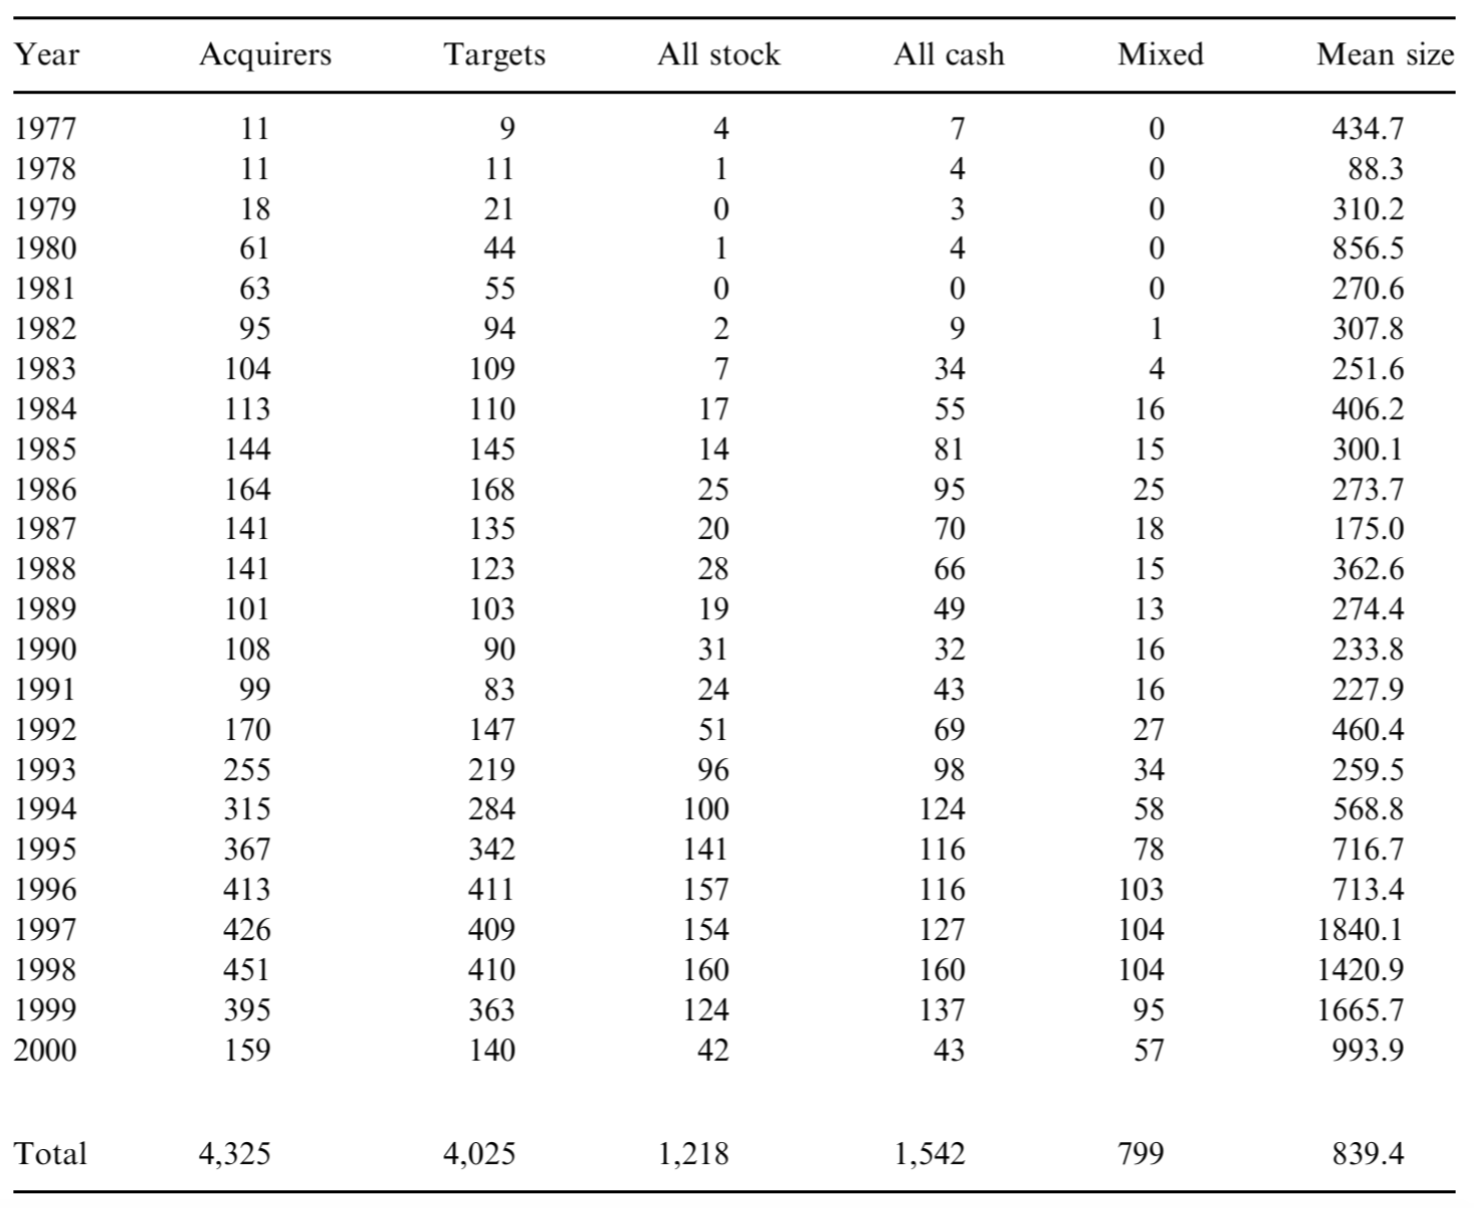
\includegraphics[width=0.55\linewidth]{figures/p2_table1.png}
        \caption{Characteristics of merger sample}
    \end{figure}
\end{frame}

\begin{frame}{Characteristics of merger and nonmerger firms}
    \begin{figure}
        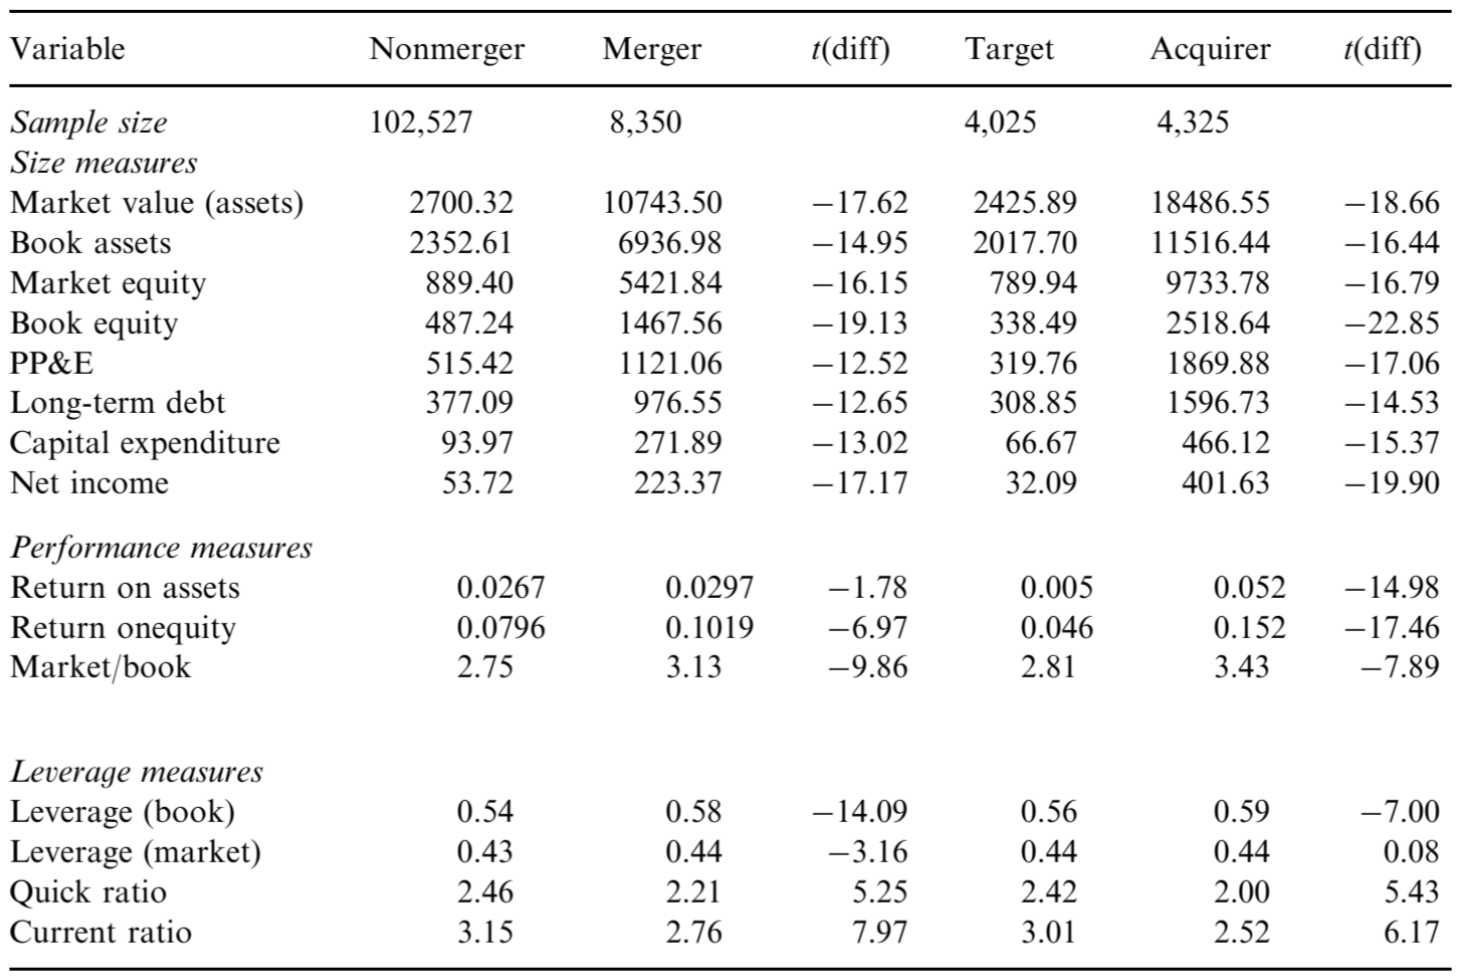
\includegraphics[width=0.7\linewidth]{figures/p2_table2.png}
        \caption{Characteristics of merger and nonmerger firms}
    \end{figure}
\end{frame}

\begin{frame}{Industrycharacteristics used in subsequent valuation models}
    \begin{figure}
        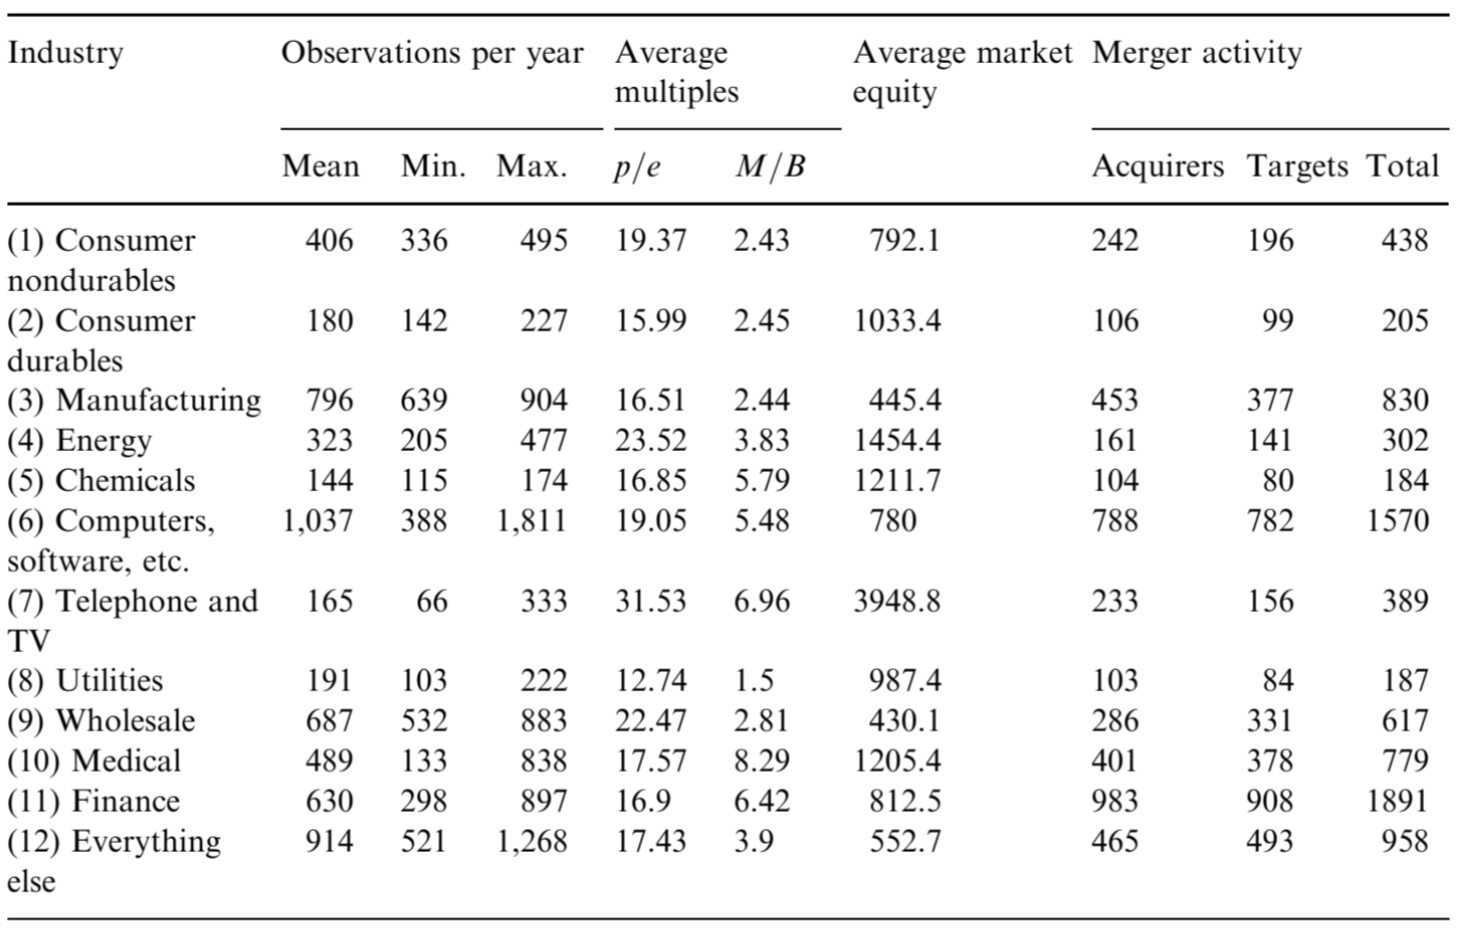
\includegraphics[width=0.8\linewidth]{figures/p2_table3.png}
        \caption{FFI12}
    \end{figure}
\end{frame}

\section{Methodologies}

\begin{frame}{Decomposing market to book}
    \begin{block}{Market value $\rightarrow$ true value $\rightarrow$ book value}
        $m - b = (m - v) + (v - b)$
        Log-linear
    \end{block}
    \begin{itemize}
        \item firm-specific error
        \item time-series sector error
        \item long-run value to book
    \end{itemize}
    \begin{equation}
        m_{i,t} - b_{i,t} = m_{i,t} - v(\theta_{i,t}; \alpha_{j,t}) + v(\theta_{i,t}; \alpha_{j,t}) - v(\theta_{i,t}; \alpha_{j}) - v(\theta_{i,t}; \alpha_j) - b_{i,t}
    \end{equation}
    $\theta_{i,t}$: firm-specific accounting information (fundamental)
\end{frame}

\begin{frame}{Estimating market value}
    \begin{block}{FCF measure}
        \begin{equation}
            M_t = \int_{t}^{\infty} e^{-\int_{t}^{\tau} r(\eta)d \eta} \textbf{FCF} d \tau
        \end{equation}
    \end{block}
    market value = book value + EVA
    RI: residual income

    \begin{equation}
        M_t = B_t + \int_{t}^{\infty} e^{-\int_{t}^{\tau} r(\eta)d \eta} \textbf{RI} d \tau
    \end{equation}
    RI = ROE - CoC
    \begin{equation}
        M_t = B_t + E_t \sum_{\tau = t+1}^{\infty} \frac{ROE_{\tau} - r_{\tau} B_{\tau - 1}}{(1+r_{\tau})^{\tau}}
    \end{equation}
\end{frame}

\begin{frame}{Model 1: market value and book value}
    \begin{block}{Identifying restriction}
        1. $E_t(ROE_t) = \lambda E_t r_\tau$ \\
        2. $B_t$ grows at a constant rate
        \begin{equation}
            m_{i,t} = \alpha_{0,j,t} + \alpha_{1,j,t} b_{i,t} + \epsilon_{i,t}
        \end{equation}
        $\alpha_{0,j,t}$: value of intangibles in average firm in industry j.
        \begin{equation}
            v(B_{i,t}; \hat{\alpha}_{0, j,t}, \hat{\alpha}_{1, j,t}) = \hat{\alpha}_{0, j,t} + \hat{\alpha}_{1, j,t} b_{i,t}
        \end{equation}

        \begin{equation}
            v(B_{i,t}; \bar{\alpha}_{0, j,t}, \bar{\alpha}_{1, j,t}) = \bar{\alpha}_{1, j,t} + \bar{\alpha}_{1, j,t} b_{i,t}
        \end{equation}
    \end{block}
\end{frame}


\begin{frame}{Model 2: market value, book value, and net income}
    \begin{block}{Identifying restriction}
        Net income grows at a constant rate
        \begin{equation}
            m_{i,t} = \alpha_{0,j,t} + \alpha_{1,j,t} b_{i,t} + \alpha_{2,j,t} ln(NI)^{+}_{i,t} + \alpha_{3,j,t} I_{(<0)} ln(NI)^{+}_{i,t} + \epsilon_{i,t}
        \end{equation}

        \begin{equation}
            v(B_{i,t}; \hat{\alpha}_{0, j,t}, \hat{\alpha}_{1, j,t}, \hat{\alpha}_{2, j,t}, \hat{\alpha}_{3, j,t}) = \hat{\alpha}_{0, j,t} + \hat{\alpha}_{1, j,t} b_{i,t} + \hat{\alpha}_{2, j,t}ln(NI)^{+}_{i,t} + \hat{\alpha}_{3, j,t} I_{(<0)} ln(NI)^{+}_{i,t}
        \end{equation}

        \begin{equation}
            v(B_{i,t}; \bar{\alpha}_{0, j,t}, \bar{\alpha}_{1, j,t}, \bar{\alpha}_{2, j,t}, \bar {\alpha}_{3, j,t}) = \bar {\alpha}_{0, j,t} + \bar {\alpha}_{1, j,t} b_{i,t} + \bar {\alpha}_{2, j,t}ln(NI)^{+}_{i,t} + \bar {\alpha}_{3, j,t} I_{(<0)} ln(NI)^{+}_{i,t}
        \end{equation}
    \end{block}
\end{frame}

\begin{frame}{Model 3: market value, book value, net income and leverage}
    \begin{block}{Identifying restriction}
        Leverage affects CoC
        \begin{equation}
            m_{i,t} = \alpha_{0,j,t} + \alpha_{1,j,t} b_{i,t} + \alpha_{2,j,t} ln(NI)^{+}_{i,t} + \alpha_{3,j,t} I_{(<0)} ln(NI)^{+}_{i,t} + \alpha_{4,j,t} LEV + \epsilon_{i,t}
        \end{equation}

        \begin{equation}
            v(B_{i,t}; \hat{\alpha}_{0, j,t}, \hat{\alpha}_{1, j,t}, \hat{\alpha}_{2, j,t}, \hat{\alpha}_{3, j,t}) = \hat{\alpha}_{0, j,t} + \hat{\alpha}_{1, j,t} b_{i,t} + \hat{\alpha}_{2, j,t}ln(NI)^{+}_{i,t} + \hat{\alpha}_{3, j,t} I_{(<0)} ln(NI)^{+}_{i,t} + \hat{\alpha}_{4,j,t} LEV
        \end{equation}

        \begin{equation}
            v(B_{i,t}; \bar{\alpha}_{0, j,t}, \bar{\alpha}_{1, j,t}, \bar{\alpha}_{2, j,t}, \bar {\alpha}_{3, j,t}) = \bar {\alpha}_{0, j,t} + \bar {\alpha}_{1, j,t} b_{i,t} + \bar {\alpha}_{2, j,t}ln(NI)^{+}_{i,t} + \bar {\alpha}_{3, j,t} I_{(<0)} ln(NI)^{+}_{i,t} + \bar{\alpha}_{4,j,t} LEV
        \end{equation}
    \end{block}
\end{frame}

\begin{frame}{Conditional regression multiples}
    \begin{figure}
        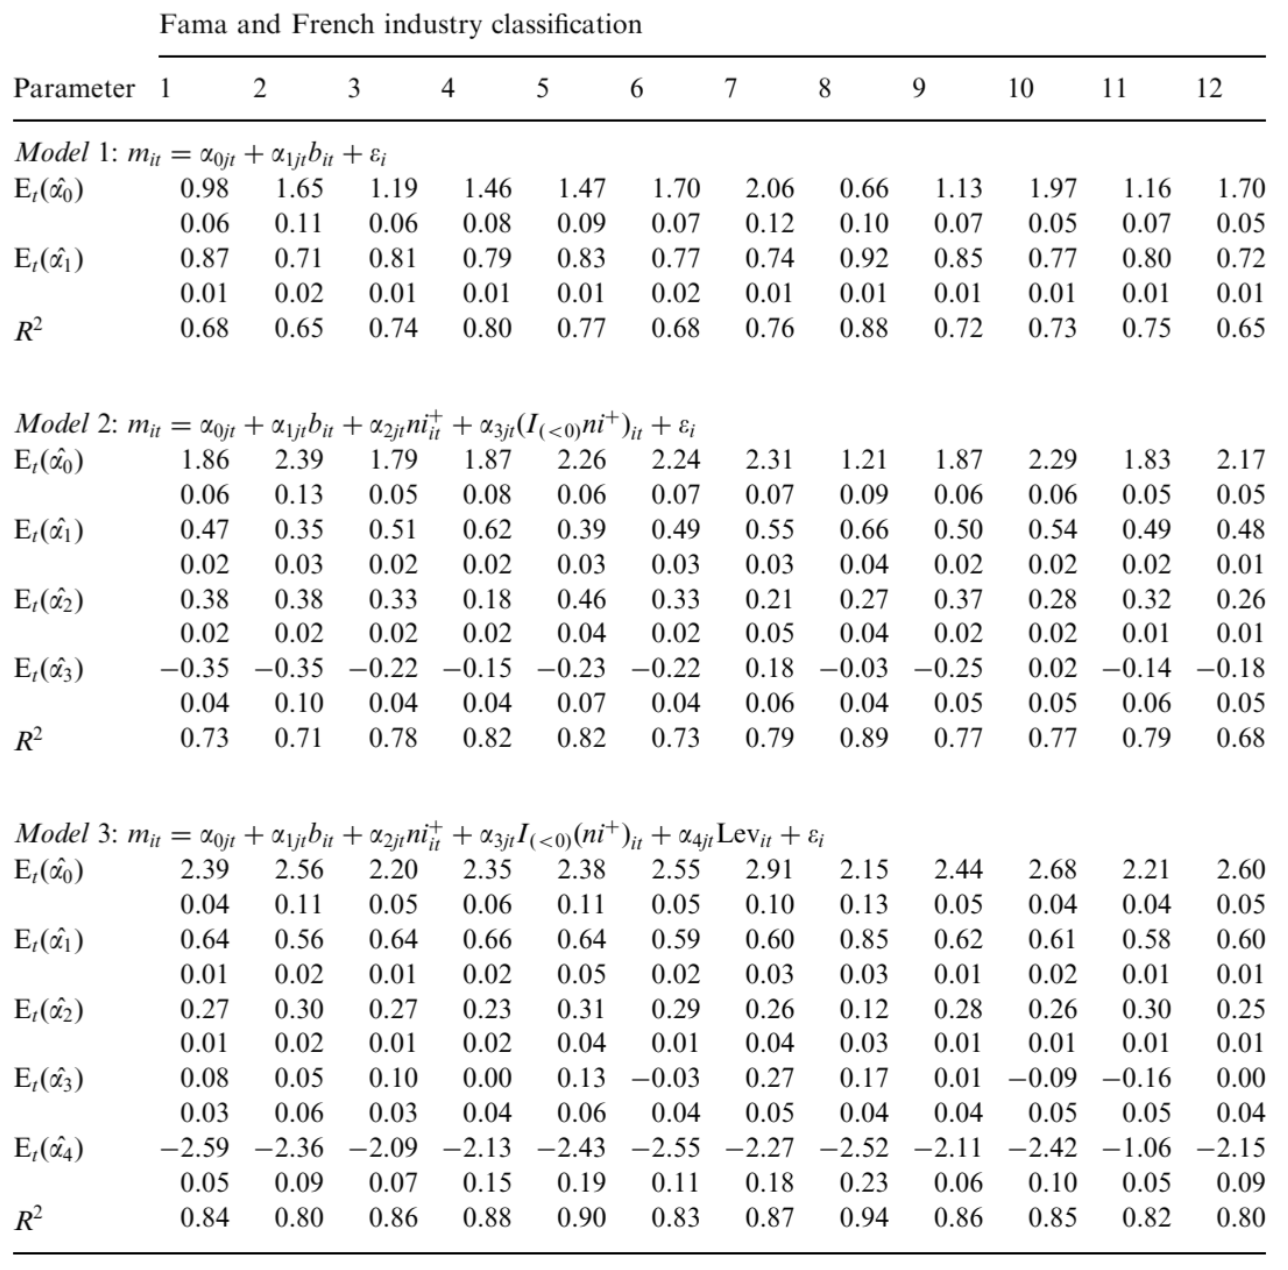
\includegraphics[width=0.55\linewidth]{figures/p2_table4.png}
        \caption{Conditional regression multiples}
    \end{figure}
\end{frame}

\begin{frame}{Components of the decomposed market-to-book ratio}
    \begin{figure}
        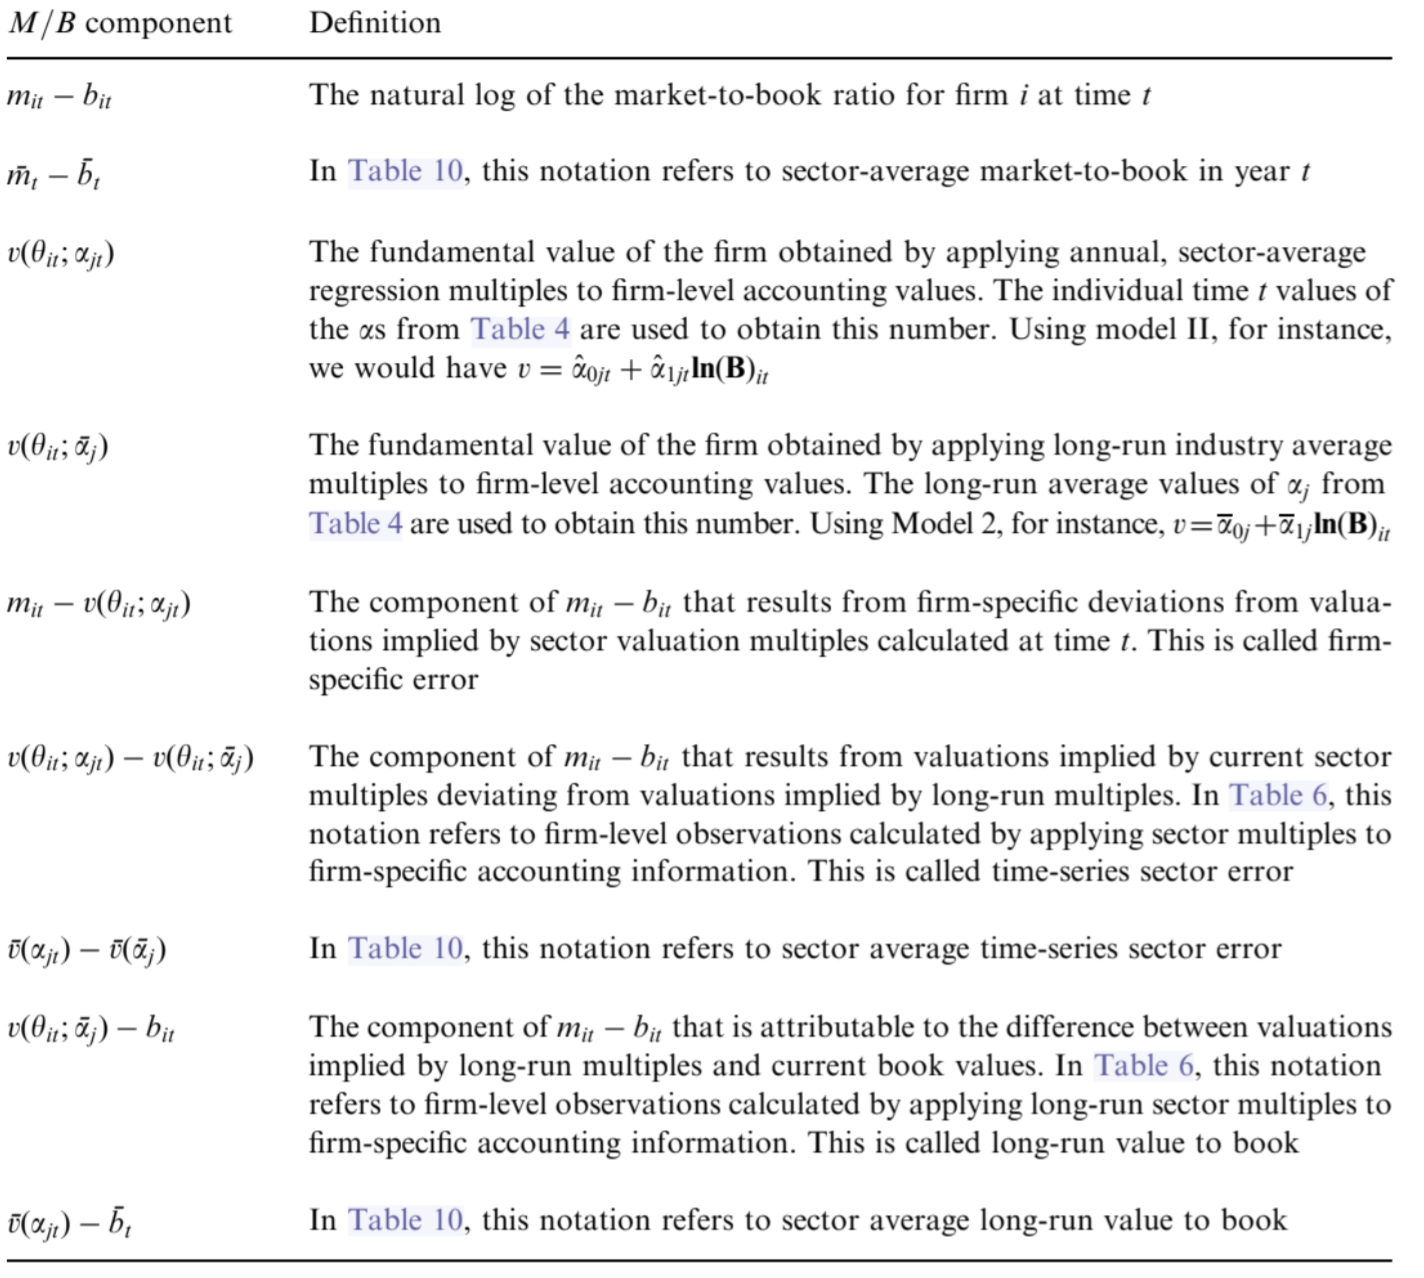
\includegraphics[width=0.55\linewidth]{figures/p2_table5.png}
        \caption{Components of the decomposed market-to-book ratio}
    \end{figure}
\end{frame}


\begin{frame}{Implication}
    \begin{block}{Everything that is not accounted for by book value, net income, and leverage is pricing error}
        Does it hold?

    \end{block}

\end{frame}

\section{Empirical results}

\begin{frame}{Deomposition of MB ratio at firm level}
    \begin{figure}
        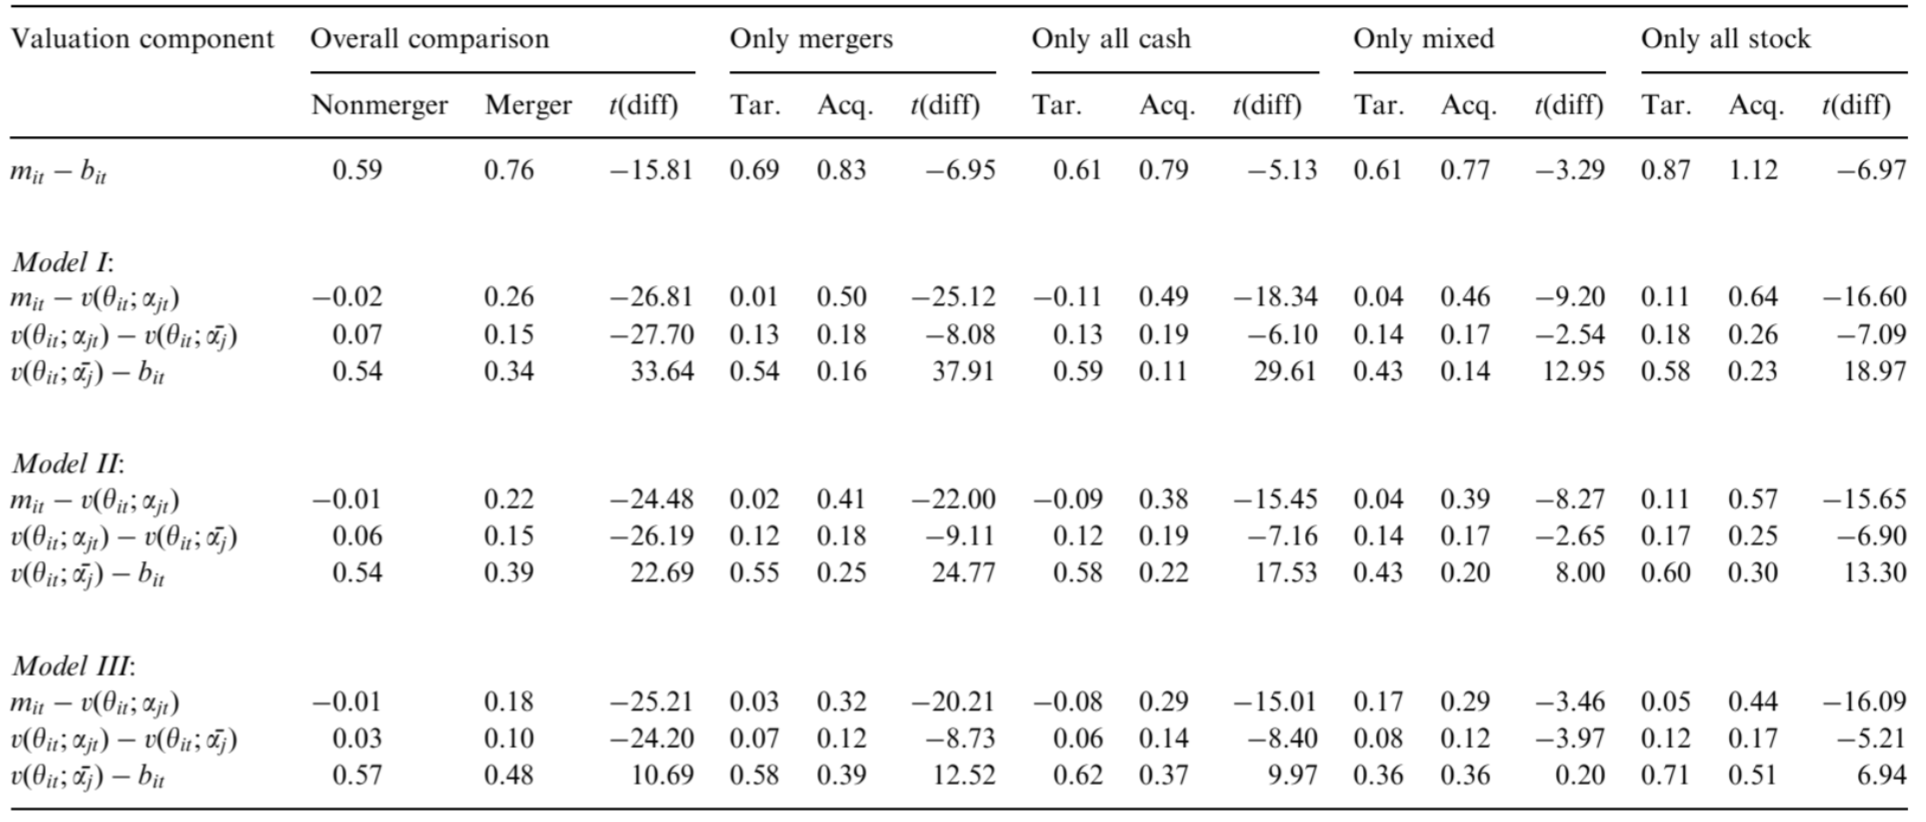
\includegraphics[width=1\linewidth]{figures/p2_table6.png}
        \caption{Deomposition of MB ratio at firm level}
    \end{figure}
\end{frame}

\begin{frame}{Robustness of firm level market-to-book decomposition}
    \begin{figure}
        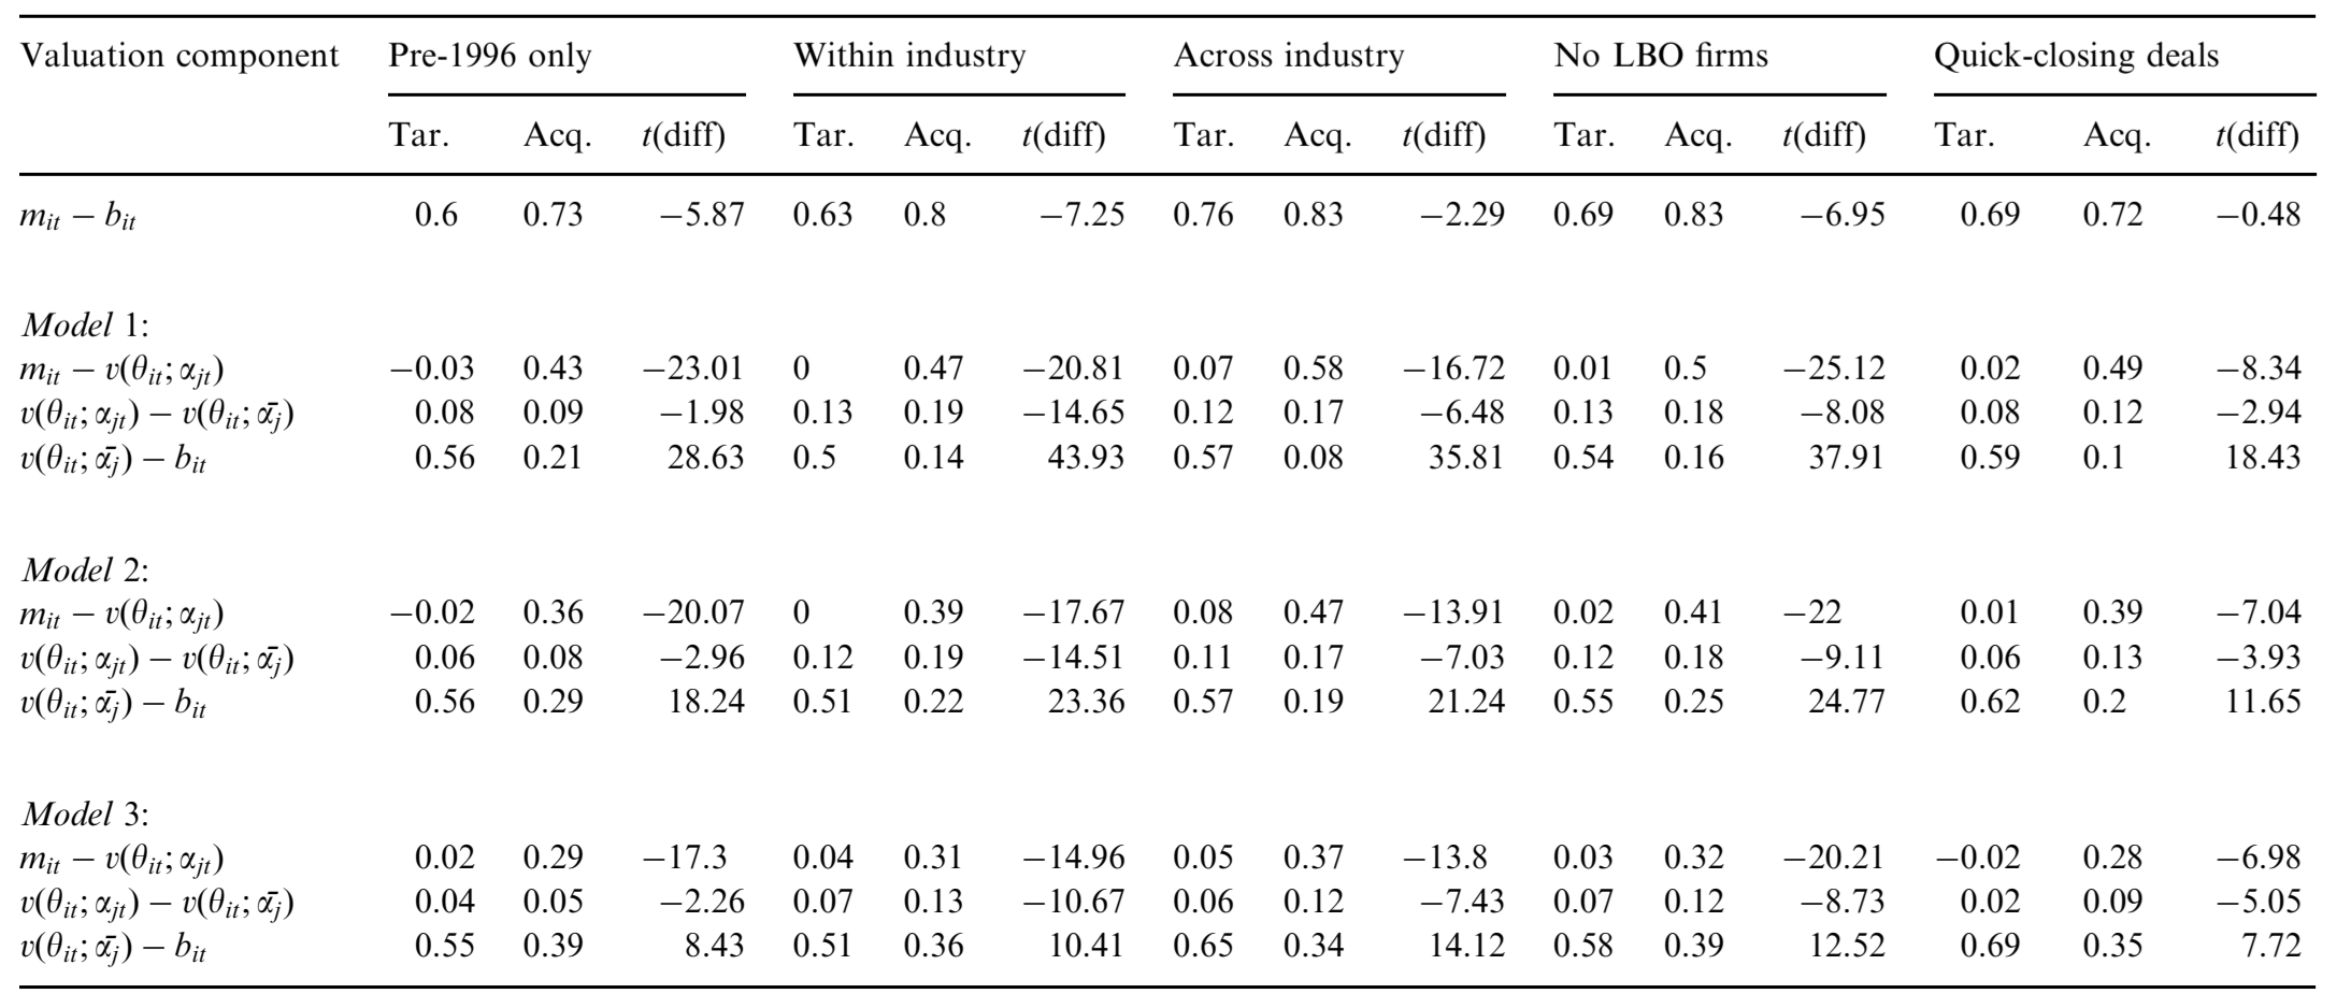
\includegraphics[width=1\linewidth]{figures/p2_table7.png}
        \caption{Robustness of firm level market-to-book decomposition}
    \end{figure}
\end{frame}

\begin{frame}{Transaction size and the components of market to book}
    \begin{figure}
        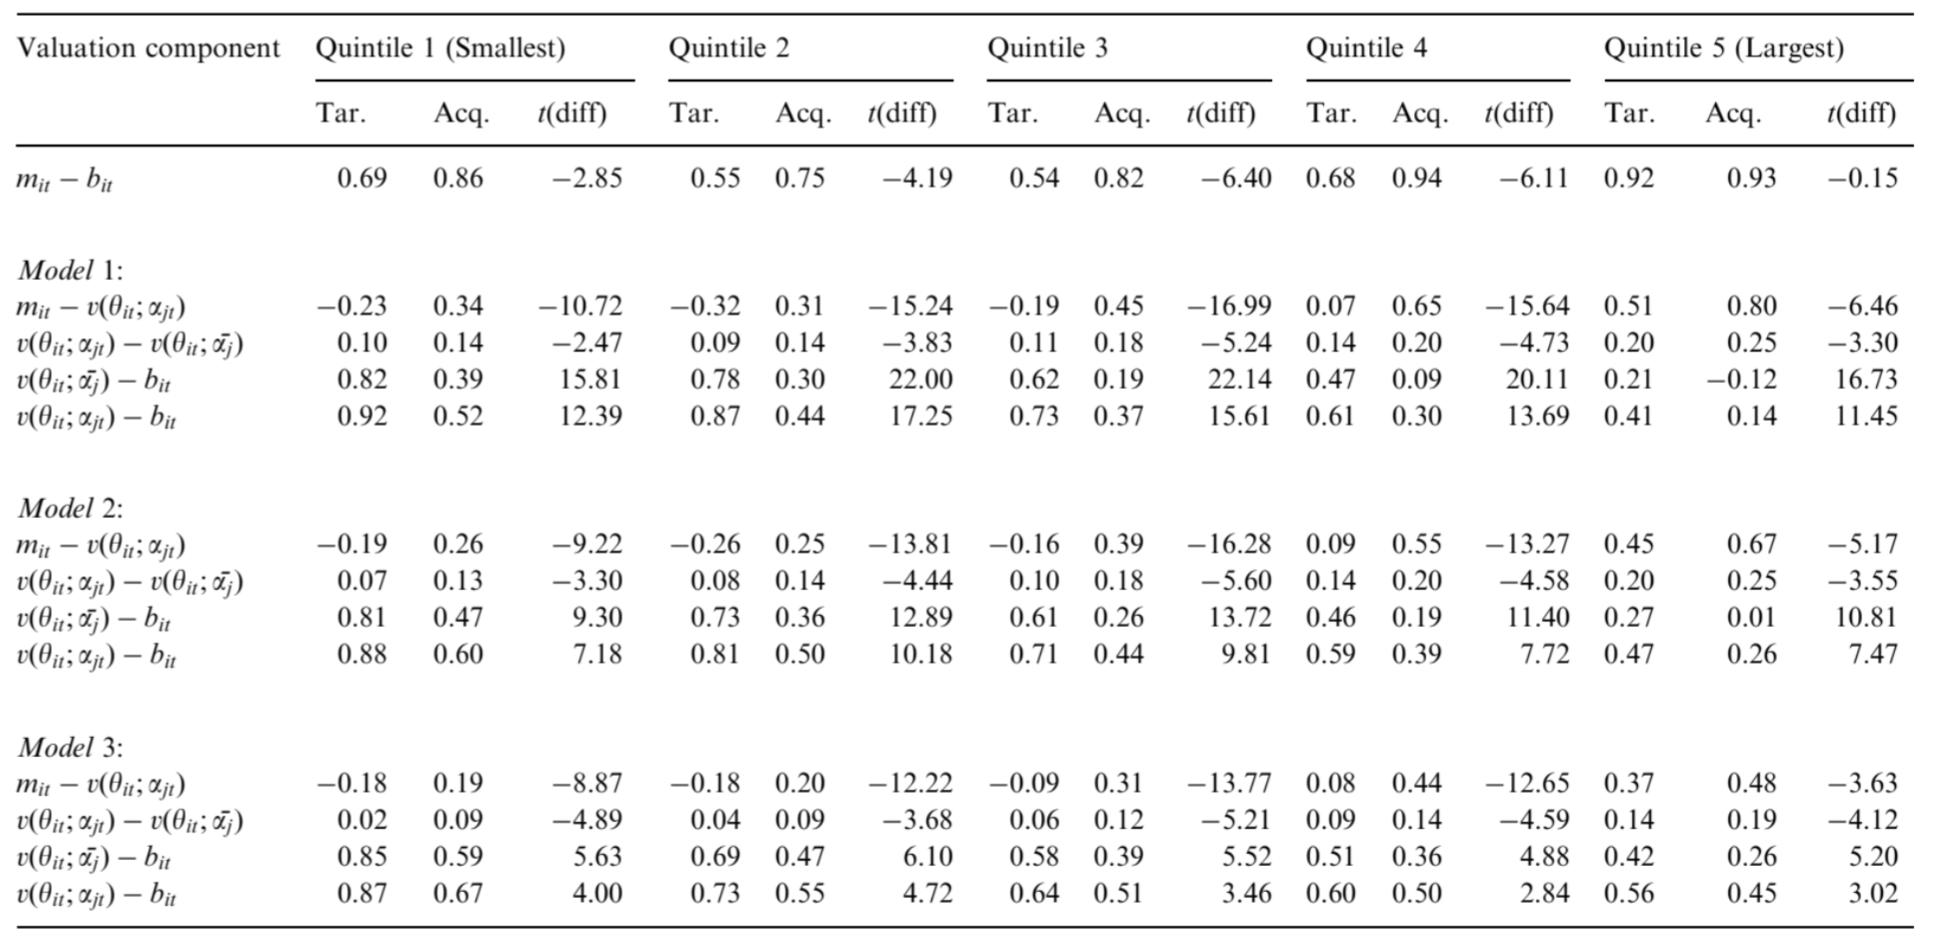
\includegraphics[width=1\linewidth]{figures/p2_table8.png}
        \caption{Transaction size and the components of market to book}
    \end{figure}
\end{frame}

\begin{frame}{Firm-level merger intensity}
    \begin{figure}
        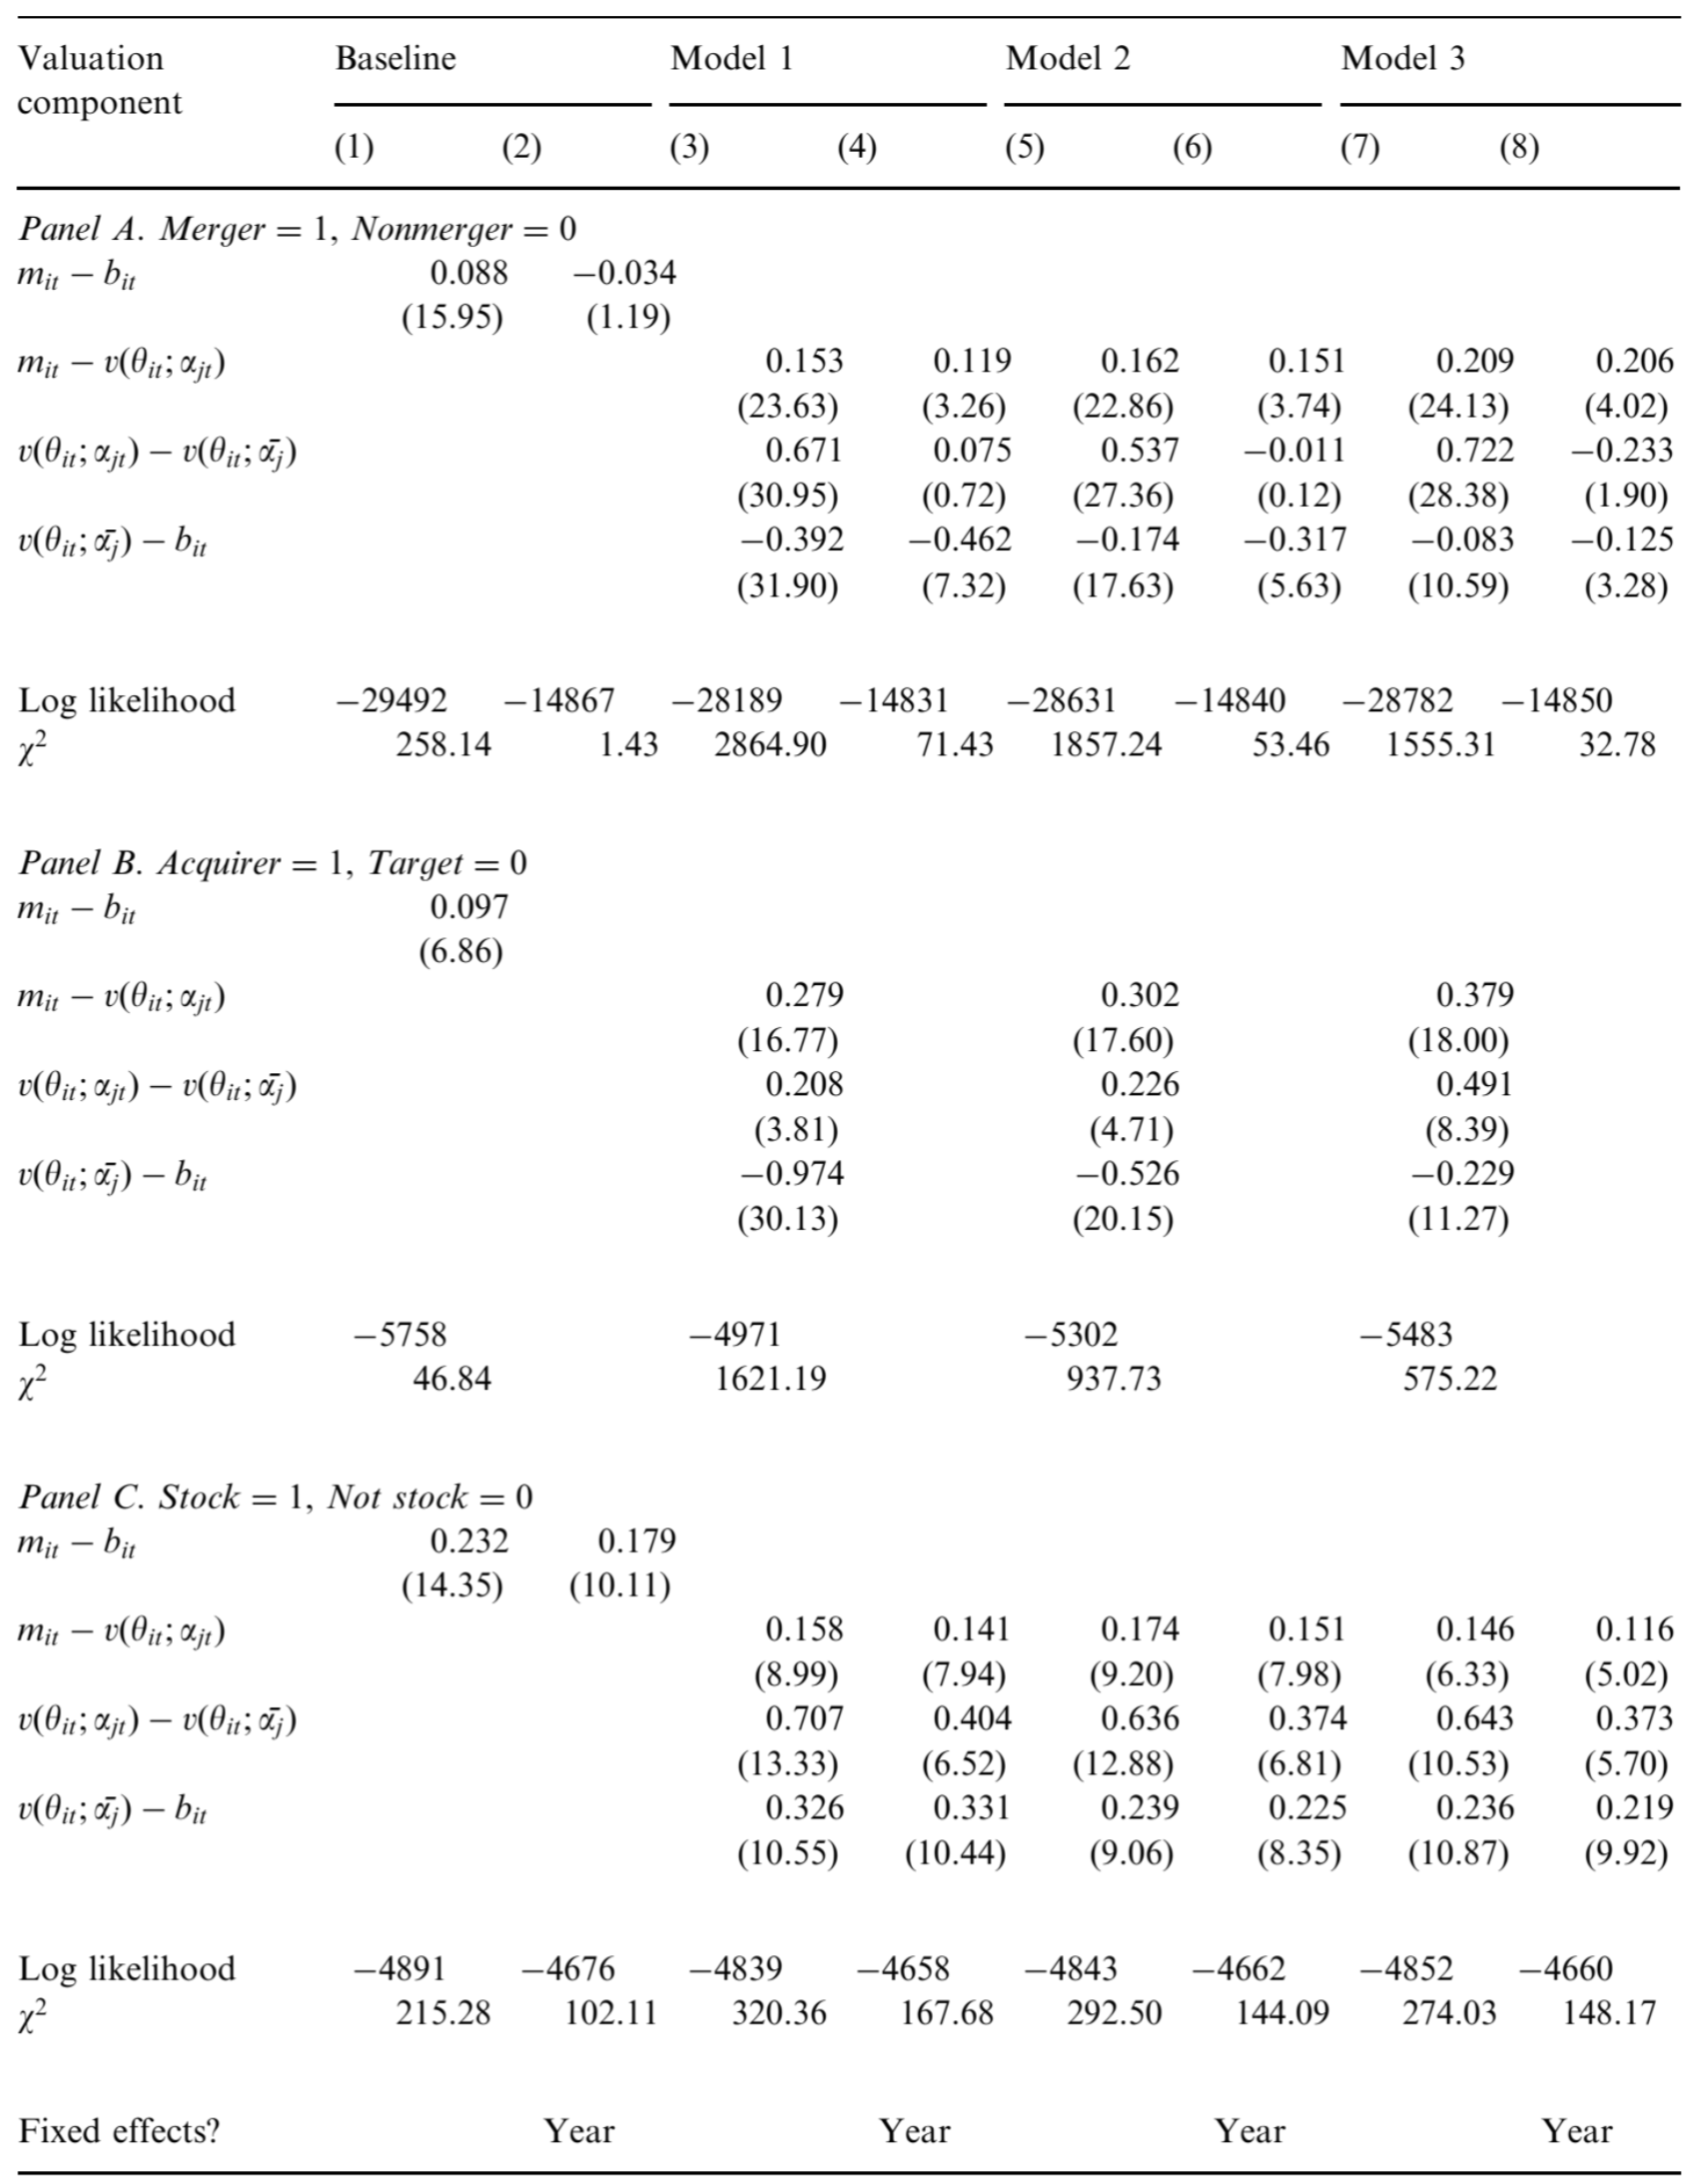
\includegraphics[width=0.4\linewidth]{figures/p2_table9.png}
        \caption{Firm-level merger intensity}
    \end{figure}
\end{frame}

\begin{frame}{Valuation waves, merger intensity, and method of payment}
    \begin{figure}
        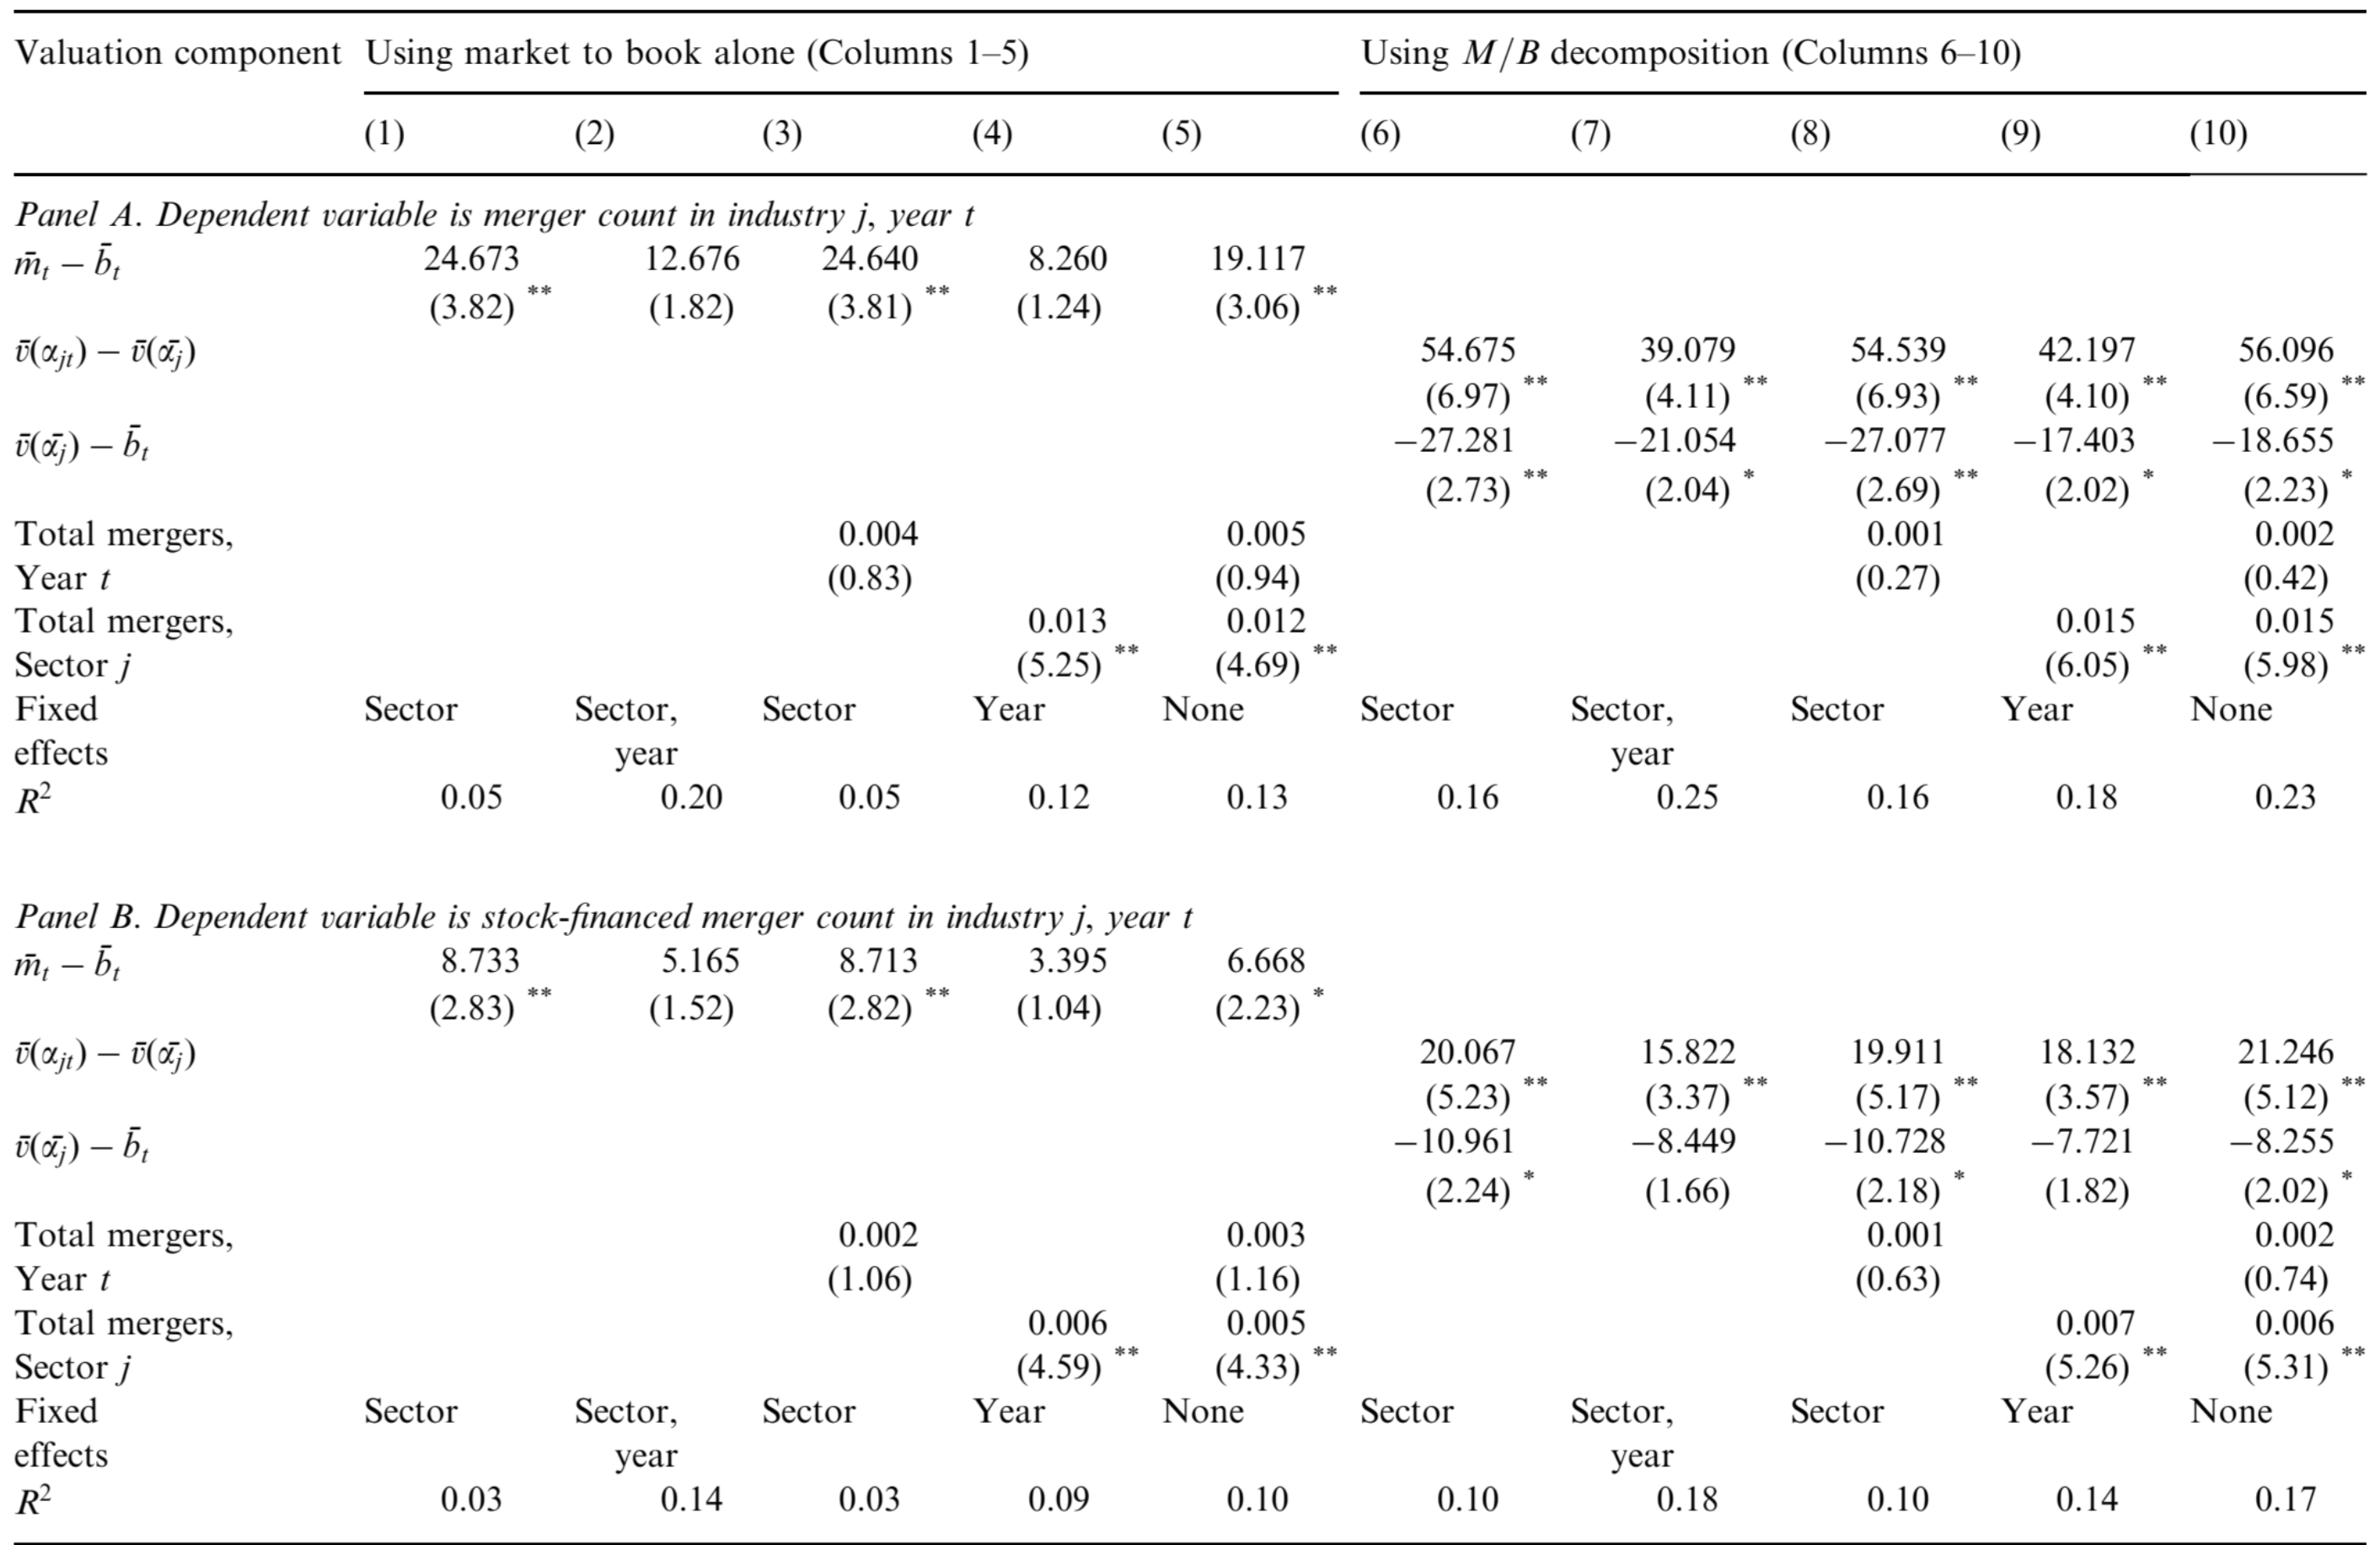
\includegraphics[width=0.8\linewidth]{figures/p2_table10.png}
        \caption{Valuation waves, merger intensity, and method of payment}
    \end{figure}
\end{frame}

\begin{frame}{Failed versus successful targets}
    \begin{figure}
        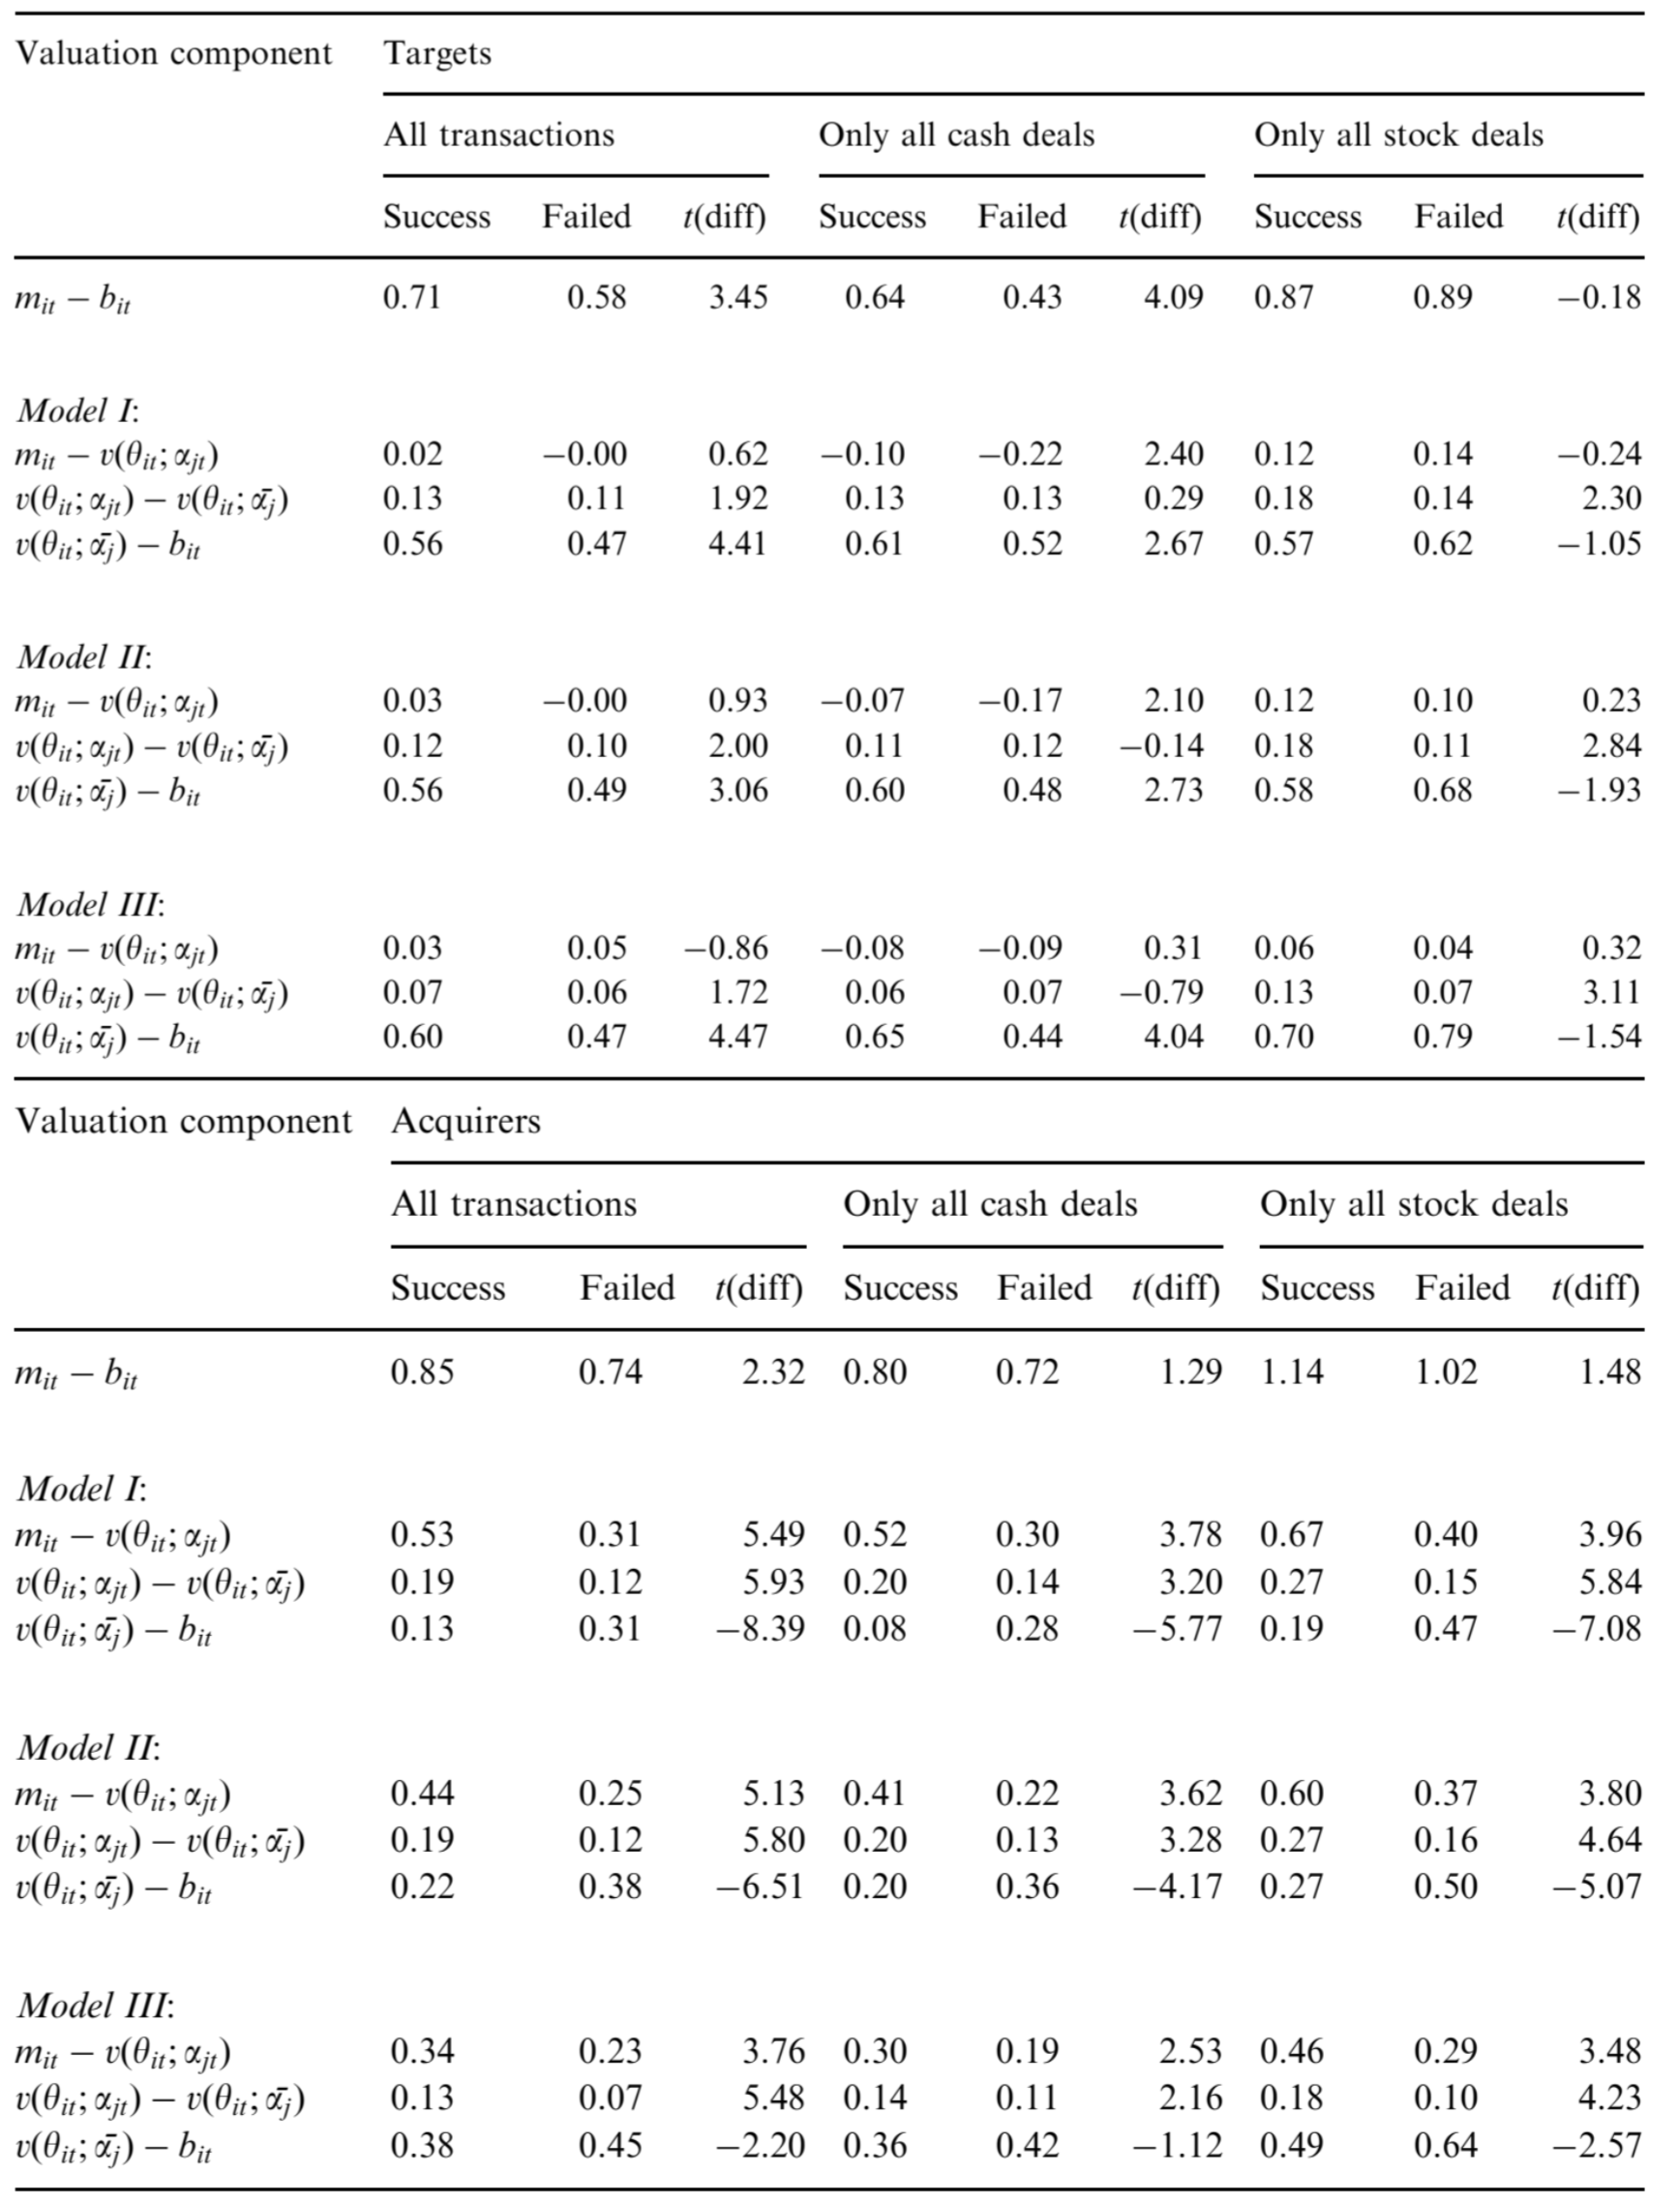
\includegraphics[width=0.4\linewidth]{figures/p2_table11.png}
        \caption{Failed versus successful targets}
    \end{figure}
\end{frame}

\begin{frame}{A horse race between competing theories of merger}
    \begin{figure}
        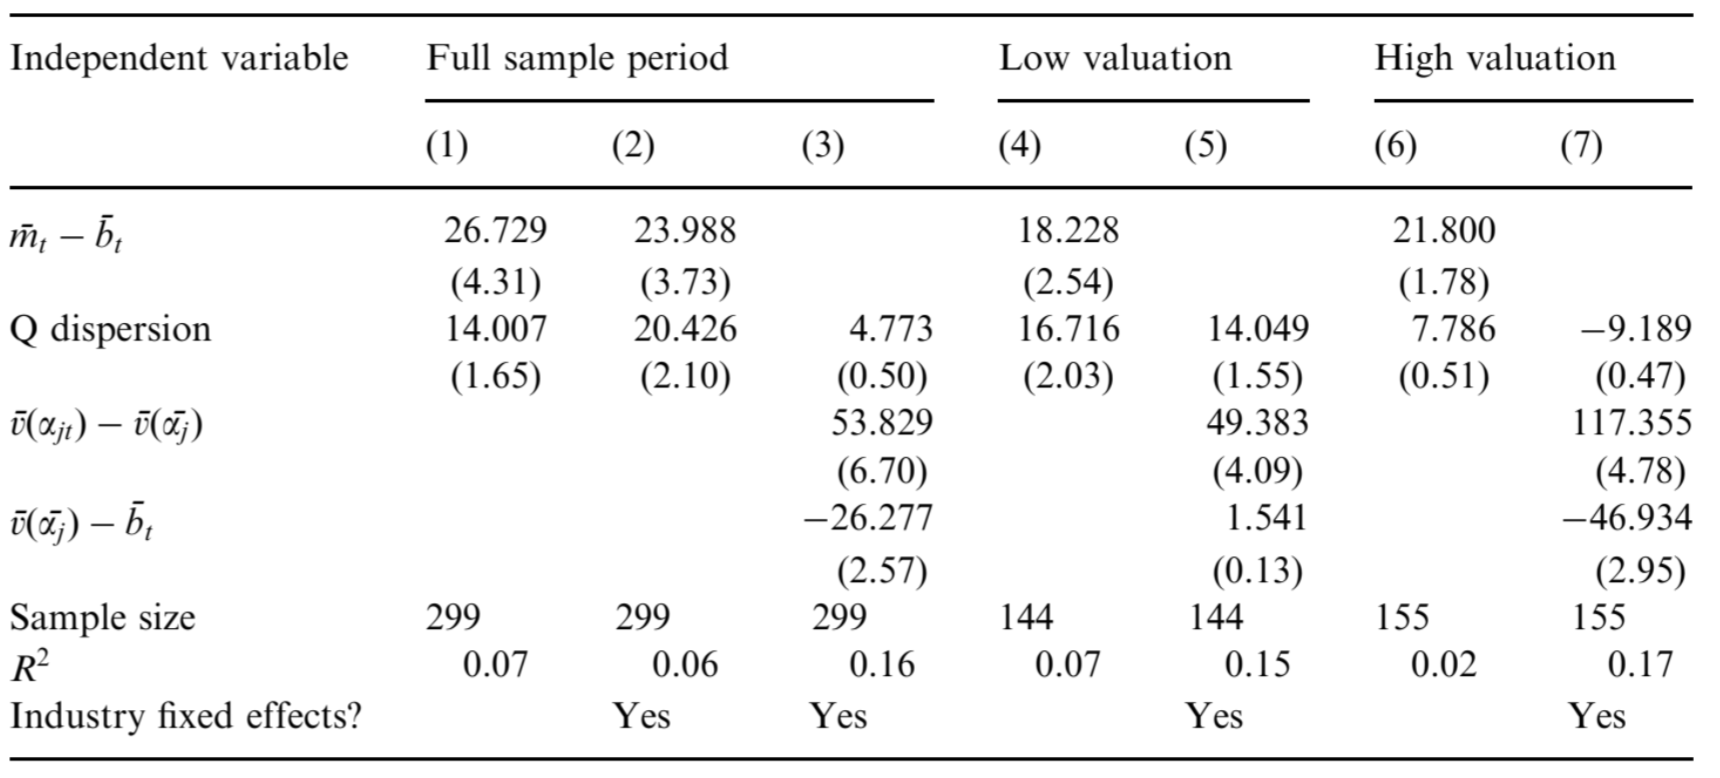
\includegraphics[width=1\linewidth]{figures/p2_table12.png}
        \caption{A horse race between competing theories of merger}
    \end{figure}
\end{frame}

\begin{frame}{Misvaluation and merger activity during economic shocks}
    \begin{figure}
        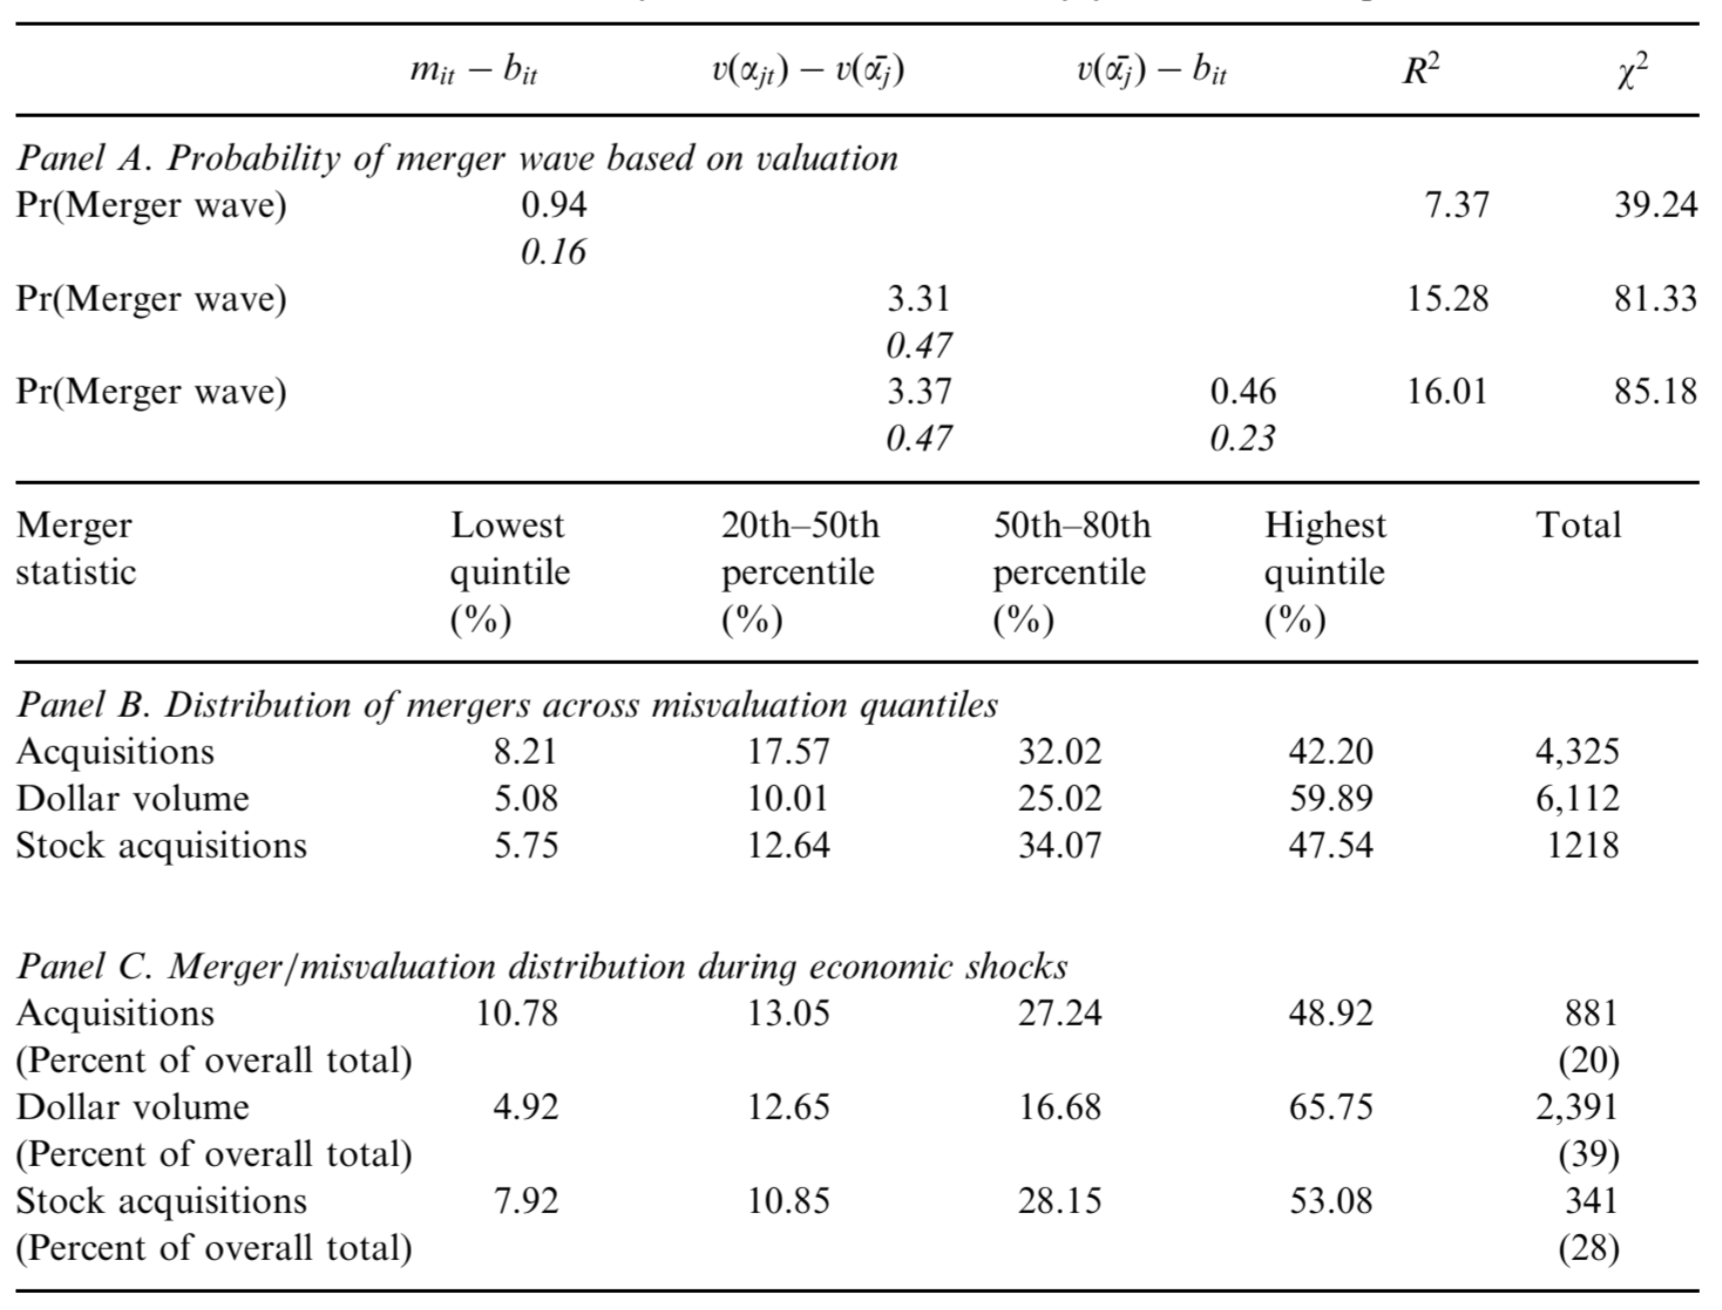
\includegraphics[width=0.7\linewidth]{figures/p2_table13.png}
        \caption{Misvaluation and merger activity during economic shocks}
    \end{figure}
\end{frame}


\section{Discussion}

\begin{frame}{Discussion}
    \begin{block}{Study is self-contained, but empirical framework not strong.}
        \begin{itemize}
            \item No clear identification strategy
            \item No clear causal relationship
            \item No clear mechanism
        \end{itemize}
    \end{block}
\end{frame}


\begin{frame}
    \Huge{\centerline{\textbf{The End}}}
\end{frame}

\end{document}